\documentclass[a4paper]{article}

\usepackage[utf8]{inputenc}
\usepackage{erk}
\usepackage{times}
\usepackage{graphicx}
\usepackage[top=22.5mm, bottom=22.5mm, left=22.5mm, right=22.5mm]{geometry}

\usepackage[slovene,english]{babel}
\usepackage{hyperref}
\usepackage{url}

\let\oldfootnotesize\footnotesize
\renewcommand*{\footnotesize}{\oldfootnotesize\scriptsize}

\begin{document}
\title{Seminarska naloga pri predmetu računališka grafika}

\author{ \large {Erazem Bršar}: \normalfont 63170066 
	\and \hspace*{-3em} \large{ Nejc Ravnik}: \normalfont 63140219  } 

\email{ Epošta: eb4311@student.uni-lj.si , nr4599@student.uni-lj.si}
\affiliation{Univerza v Ljubljani, Fakulteta za računalništvo in informatiko }
\maketitle

\selectlanguage{slovene}

\begin{abstract}{Abstract}
	Za seminarsko nalogo bova naredila 3D igro, kjer se igralec postavi v vlogo taksista. Njegov cilj bo, da v čim krajšem času pobere stranko in jo pripelje na željen cilj. Na njegovi vožnji se pojavljajo ovire (avtomobili, delo na cesti, pešci..) in, če se zadane ob njih poškoduje svoj taksi in dobi denarno kazen. Po uspešnem prevozu potnika mu ta glede na prevoženo razdaljo in kvaliteto vožnje(igralec se mora čim manjkrat zaleteti v ovire) plača določeno vsoto denarja. Ta denar lahko igralec porabi za odplačevanje kazni, popravilo taksija ali pa za izboljšavo le tega\end{abstract}



\section{Pregled igre}
Gre ze dirkaško igro. kjer voziš avto po ustvarjenem svetu. Mišljeno je bilo da bo ustvarjen taxi ki bo pobiral ljudi, pa nama ni uspelo priti tako daleč-

\subsection{Opis sveta}
Svet je sestavljen iz ceste okoli katere so zidovi.
\begin{figure}[!htb]
	\begin{center}
		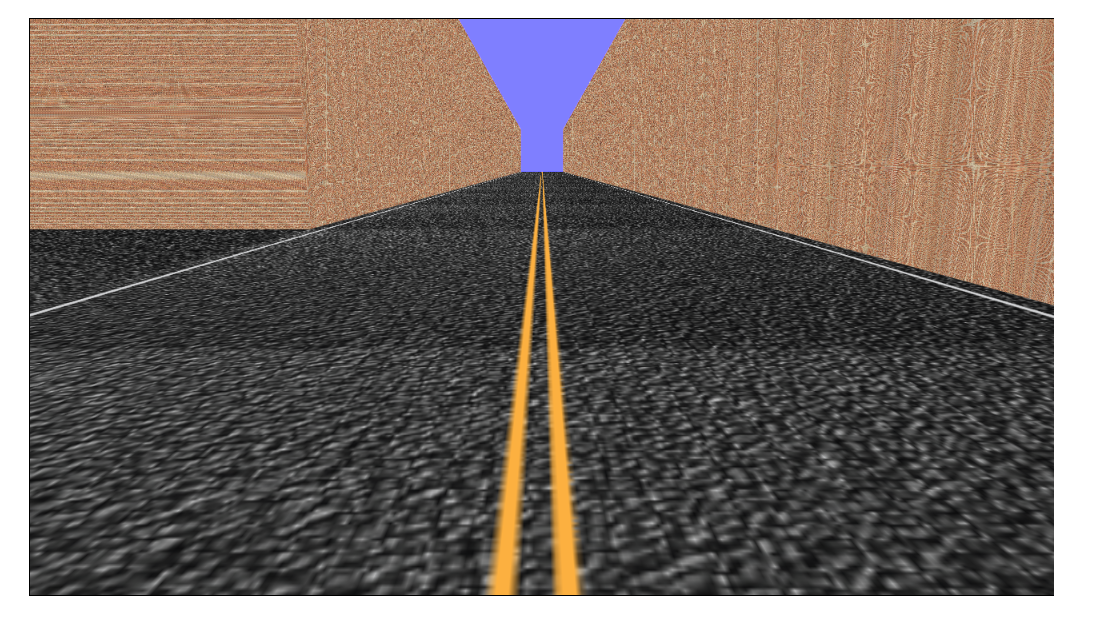
\includegraphics[width=\columnwidth]{ozadje.png}
		\caption{Screenshot iz igre} \label{fig:slika}
	\end{center}
\end{figure}

\subsubsection{Pregled}
Uporabnik ima na voljo navizedni svet po katerem se vozi z avtomobilom kot da ga vozi za volanom. Vmes lahko zavijo po križiščih.Okolje sva generirala s pomočjo datotek, v katere sva napisala koordinate ter jih povezala z ustreznimi teksturami

\subsubsection{Ozadje}
Ozadje je nebo. Predstavljeno je z modro barvo

\subsubsection{Ključne lokacije}
Ključna lokacija je navidezni prostor obdan s stenami in cesto.


\subsubsection{Velikost}
Svet je pravokotnik in ima obseg takšen kot ce greš po glavni  cesti (brez da zavijas tam ko ni treba) vendar se lahko uporabnik premika le po cesti.

\subsubsection{Objekti}
Poglavitni objekti so kamera(predstavljena skozi oči uporabnika, ki se vozi po cesti), zidovi ter tla(cesta).

\subsubsection{Čas}
Čas v tej verziji igre še  ni dolocen, zato se igrica lahko igra v neskoncnost.

\subsection{Igralni pogon in uporabljene tehnologije}
Uporabljeno je bil webGL, ter javascript. Pomagala pa sva si z urejevalnikom JetBrains Webstorm IDE. Za pomoč pri igri sva uporabila knjižnico glMatrix.

\subsection{Pogled}
Pogled je prvoosebni, uporabnk  vidi cesto ter zidove.Uporabnik lahko vidi le do določene globine. Kar je bolj oddaljeno od tega se ne izriše, na tem mestu uporabnik vidi ozadje(nebo).

\section{Osebek}
Osebek je clovek ki vozi avto(se ga ne vidi - ni implementiran, sam nama je za implementacijo le tega zmanjkalo časa)Ima nadzor nad premikanjem.Premika se s pomočjo tipk na tipkovnici(WASD) Lahko se premika naprej, nazaj, levo in desno.

\section{Uporabniški vmesnik}
Za uporabniški vmesnik je izbrano platno webGL.

\section{Glasba in zvok}
V tej verziji igre zvok in glasba še nista dodana.

\section{Gameplay}
Igra je neskončna. Igra se prične tako, da je uporabnik postavljen na cesto in se nato lahko vozi po njej. Ni nobenega cilja, uporabnik ima prosto izbiro po kateri cesti se bo premikal.



\section{Zaključki in možne nadgradnje}
Končna igra ni enaka kot zasnovana. Zasnovano je bilo da bo uporabnik pobiral potnike in jih pripeljal na cilj.
Naučila sva se uporabljati teksture in ustvariti navidezno okolje. Pri izdelavi igre sva slabo precenila čaš kibi bi si ga morala vzeti za implementacijo ideje ki sva si jo zadala na začetku. Veliko pa sva odnesla in se pri izdelavi vseeno naučila zlasti s pomočjo asistentovih videov.


\small
\bibliographystyle{plain}

\bibliography{references}

\href{https://www.khronos.org/webgl/wiki/Main_Pag}{WebGlWiki:https://www.khronos.org/webgl/}


\href{http://glmatrix.net/}{GLMatrix:http://glmatrix.net/}

\href{https://www.youtube.com/watch?v=AsKf-BQqIk4&list=PLpOjccKU6Yiz4tcDpOqaZdPQGP8gfaWQr}{WEBGL EXAMPLES}

\end{document}


